\documentclass[border=5mm]{standalone}
\usepackage{tikz}
\usetikzlibrary{calc, angles, quotes, arrows.meta}

\begin{document}
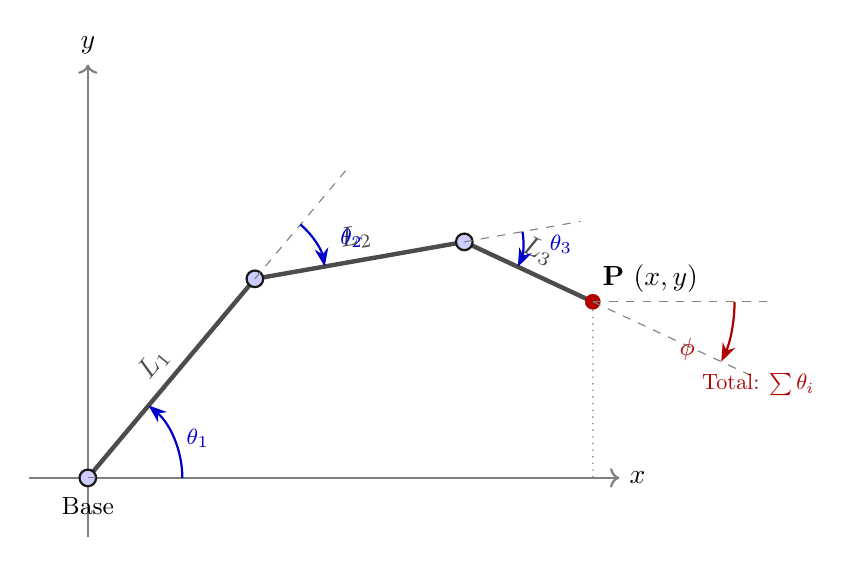
\begin{tikzpicture}[
    scale=1.5,
    link/.style={ultra thick, black!70, line cap=round},
    joint/.style={circle, draw=black!90, fill=blue!20, thick, inner sep=2pt, minimum size=6pt},
    endeffector/.style={circle, fill=red!70!black, inner sep=2pt}
]

    % Longitudes de los eslabones
    \def\Lone{2.2}
    \def\Ltwo{1.8}
    \def\Lthree{1.2}
    
    % Ángulos (grados)
    \def\thetaone{50}
    \def\thetatwo{-40}
    \def\thetathree{-35}

    % Cálculo matemático de las coordenadas
    \coordinate (O) at (0,0);
    \coordinate (J1) at (\thetaone:\Lone);
    \coordinate (J2) at ($ (J1) + (\thetaone+\thetatwo:\Ltwo) $);
    \coordinate (EE) at ($ (J2) + (\thetaone+\thetatwo+\thetathree:\Lthree) $);

    % Dibujo de Ejes de Referencia Global
    \draw[->, thick, gray] (-0.5, 0) -- (4.5, 0) node[right, text=black] {$x$};
    \draw[->, thick, gray] (0, -0.5) -- (0, 3.5) node[above, text=black] {$y$};

    % Trazado de los Eslabones con etiquetas separadas
    \draw[link] (O) -- (J1) node[midway, sloped, above] {$L_1$};
    \draw[link] (J1) -- (J2) node[midway, sloped, above] {$L_2$};
    \draw[link] (J2) -- (EE) node[midway, sloped, above] {$L_3$};

    % Nodos de las Articulaciones
    \node[joint, label=below:{\small Base}] at (O) {};
    \node[joint] at (J1) {};
    \node[joint] at (J2) {};
    \node[endeffector] (P) at (EE) {};
    \node[above right] at (P) {\textbf{P} $(x, y)$};

    % ÁNGULOS RELATIVOS (Thetas)
    % Referencia para theta 1
    \draw[dashed, gray] (O) -- (1.5,0);
    \draw[-{Stealth}, thick, blue!80!black] (0.8,0) arc (0:\thetaone:0.8) node[midway, right=1pt] {\footnotesize $\theta_1$};

    % Referencia para theta 2 (con offset para no encimar con L2)
    \draw[dashed, gray] (J1) -- ($ (J1) + (\thetaone:1.2) $);
    \draw[-{Stealth}, thick, blue!80!black] ($ (J1) + (\thetaone:0.6) $) arc (\thetaone:\thetaone+\thetatwo:0.6) node[midway, right=5pt, yshift=2pt] {\footnotesize $\theta_2$};

    % Referencia para theta 3 (con offset para no encimar con L3)
    \draw[dashed, gray] (J2) -- ($ (J2) + (\thetaone+\thetatwo:1) $);
    \draw[-{Stealth}, thick, blue!80!black] ($ (J2) + (\thetaone+\thetatwo:0.5) $) arc (\thetaone+\thetatwo:\thetaone+\thetatwo+\thetathree:0.5) node[midway, right=6pt, yshift=2pt] {\footnotesize $\theta_3$};
    
    % ÁNGULO GLOBAL PHI (Orientación total)
    % Se mide desde la horizontal hasta el último eslabón
    \draw[dashed, gray] (EE) -- ($ (EE) + (1.5, 0) $);
    \draw[dashed, gray] (EE) -- ($ (EE) + (\thetaone+\thetatwo+\thetathree:1.5) $);
    \draw[{Stealth}-, thick, red!70!black] ($ (EE) + (\thetaone+\thetatwo+\thetathree:1.2) $) arc (\thetaone+\thetatwo+\thetathree:0:1.2);
    \node[red!70!black] at ($ (EE) + (0.8, -0.4) $) {\small $\phi$};
    \node[red!70!black, scale=0.8] at ($ (EE) + (1.4, -0.7) $) {Total: $\sum \theta_i$};

    % Proyecciones cinemática directa
    \draw[dotted, gray] (P) -- (EE |- 0,0);
    \draw[dotted, gray] (P) -- (0,0 -| EE);

\end{tikzpicture}
\end{document}
